\documentclass[crop,tikz]{standalone}
\usepackage[utf8]{inputenc}
\usepackage{tikz}
\usepackage{pgfplots}
\usepackage{bm}
\pgfplotsset{compat=newest}
\usepgfplotslibrary{groupplots}


\pgfplotsset{
    legend image with color/.style={
        legend image code/.code={%
            \node[anchor=center, rectangle, fill=#1] at (0.3cm,0cm) {};
        }
    },
}
\def\fontscale{.8}

\begin{document}
% This file was created by tikzplotlib v0.8.2.
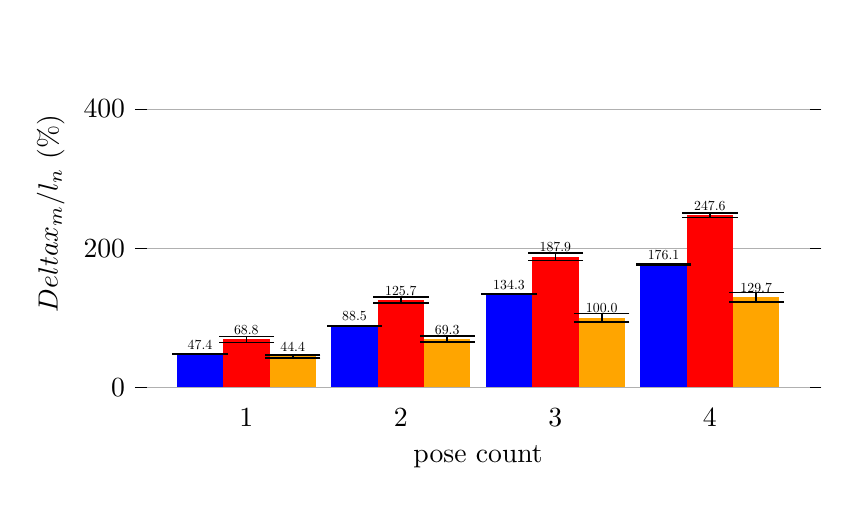
\begin{tikzpicture}
\definecolor{color0}{rgb}{1,0.647058823529412,0}
\begin{axis}[
anchor=origin,
axis line style={draw=none},
height=6cm,
legend cell align={left},
legend style={draw=white!80.0!black},
tick align=outside,
tick pos=both,
width=10cm,
x grid style={white!69.01960784313725!black},
xlabel={pose count},
xmin=-0.645, xmax=3.645,
xtick style={color=black},
xtick style={draw=none},
xtick={0,1,2,3},
xticklabels={1,2,3,4},
y grid style={white!69.01960784313725!black},
ylabel={\(\displaystyle Delta x_m/l_n\) (\%)},
ymajorgrids,
ymin=0, ymax=500,
ytick style={color=black}
]
\draw[fill=blue,draw opacity=0] (axis cs:-0.45,0) rectangle (axis cs:-0.15,47.4098407090574);
\draw[fill=blue,draw opacity=0] (axis cs:0.55,0) rectangle (axis cs:0.85,88.5194699411992);
\draw[fill=blue,draw opacity=0] (axis cs:1.55,0) rectangle (axis cs:1.85,134.295014385611);
\draw[fill=blue,draw opacity=0] (axis cs:2.55,0) rectangle (axis cs:2.85,176.12281406058);
\draw[fill=red,draw opacity=0] (axis cs:-0.15,0) rectangle (axis cs:0.15,68.8223560945423);
\draw[fill=red,draw opacity=0] (axis cs:0.85,0) rectangle (axis cs:1.15,125.731627580536);
\draw[fill=red,draw opacity=0] (axis cs:1.85,0) rectangle (axis cs:2.15,187.87789066267);
\draw[fill=red,draw opacity=0] (axis cs:2.85,0) rectangle (axis cs:3.15,247.606750771043);
\draw[fill=color0,draw opacity=0] (axis cs:0.15,0) rectangle (axis cs:0.45,44.4486221474503);
\draw[fill=color0,draw opacity=0] (axis cs:1.15,0) rectangle (axis cs:1.45,69.2960007482785);
\draw[fill=color0,draw opacity=0] (axis cs:2.15,0) rectangle (axis cs:2.45,99.9673772778017);
\draw[fill=color0,draw opacity=0] (axis cs:3.15,0) rectangle (axis cs:3.45,129.664152210846);
\path [draw=black, semithick]
(axis cs:-0.3,47.0272529027865)
--(axis cs:-0.3,47.7924285153284);
\path [draw=black, semithick]
(axis cs:0.7,88.0904077549042)
--(axis cs:0.7,88.9485321274942);
\path [draw=black, semithick]
(axis cs:1.7,133.812458207806)
--(axis cs:1.7,134.777570563416);
\path [draw=black, semithick]
(axis cs:2.7,175.169796534097)
--(axis cs:2.7,177.075831587063);
\path [draw=black, semithick]
(axis cs:0,64.3332476094806)
--(axis cs:0,73.311464579604);
\path [draw=black, semithick]
(axis cs:1,121.583596092592)
--(axis cs:1,129.879659068481);
\path [draw=black, semithick]
(axis cs:2,182.427014687371)
--(axis cs:2,193.328766637968);
\path [draw=black, semithick]
(axis cs:3,244.1730649449)
--(axis cs:3,251.040436597186);
\path [draw=black, semithick]
(axis cs:0.3,42.6123299793238)
--(axis cs:0.3,46.2849143155769);
\path [draw=black, semithick]
(axis cs:1.3,64.9242068327622)
--(axis cs:1.3,73.6677946637949);
\path [draw=black, semithick]
(axis cs:2.3,93.7304882189099)
--(axis cs:2.3,106.204266336693);
\path [draw=black, semithick]
(axis cs:3.3,123.000872262272)
--(axis cs:3.3,136.32743215942);
\addplot [semithick, black, mark=-, mark size=10, mark options={solid}, only marks, forget plot]
table {%
-0.3 47.0272529027865
0.7 88.0904077549042
1.7 133.812458207806
2.7 175.169796534097
};
\addplot [semithick, black, mark=-, mark size=10, mark options={solid}, only marks, forget plot]
table {%
-0.3 47.7924285153284
0.7 88.9485321274942
1.7 134.777570563416
2.7 177.075831587063
};
\addplot [semithick, black, mark=-, mark size=10, mark options={solid}, only marks, forget plot]
table {%
0 64.3332476094806
1 121.583596092592
2 182.427014687371
3 244.1730649449
};
\addplot [semithick, black, mark=-, mark size=10, mark options={solid}, only marks, forget plot]
table {%
0 73.311464579604
1 129.879659068481
2 193.328766637968
3 251.040436597186
};
\addplot [semithick, black, mark=-, mark size=10, mark options={solid}, only marks, forget plot]
table {%
0.3 42.6123299793238
1.3 64.9242068327622
2.3 93.7304882189099
3.3 123.000872262272
};
\addplot [semithick, black, mark=-, mark size=10, mark options={solid}, only marks, forget plot]
table {%
0.3 46.2849143155769
1.3 73.6677946637949
2.3 106.204266336693
3.3 136.32743215942
};
\node at (axis cs:-0.3,47.4)[
  scale=0.5,
  anchor=south,
  text=black,
  rotate=0.0
]{47.4};
\node at (axis cs:0.7,88.5)[
  scale=0.5,
  anchor=south,
  text=black,
  rotate=0.0
]{88.5};
\node at (axis cs:1.7,134.3)[
  scale=0.5,
  anchor=south,
  text=black,
  rotate=0.0
]{134.3};
\node at (axis cs:2.7,176.1)[
  scale=0.5,
  anchor=south,
  text=black,
  rotate=0.0
]{176.1};
\node at (axis cs:0,68.8)[
  scale=0.5,
  anchor=south,
  text=black,
  rotate=0.0
]{68.8};
\node at (axis cs:1,125.7)[
  scale=0.5,
  anchor=south,
  text=black,
  rotate=0.0
]{125.7};
\node at (axis cs:2,187.9)[
  scale=0.5,
  anchor=south,
  text=black,
  rotate=0.0
]{187.9};
\node at (axis cs:3,247.6)[
  scale=0.5,
  anchor=south,
  text=black,
  rotate=0.0
]{247.6};
\node at (axis cs:0.3,44.4)[
  scale=0.5,
  anchor=south,
  text=black,
  rotate=0.0
]{44.4};
\node at (axis cs:1.3,69.3)[
  scale=0.5,
  anchor=south,
  text=black,
  rotate=0.0
]{69.3};
\node at (axis cs:2.3,100)[
  scale=0.5,
  anchor=south,
  text=black,
  rotate=0.0
]{100.0};
\node at (axis cs:3.3,129.7)[
  scale=0.5,
  anchor=south,
  text=black,
  rotate=0.0
]{129.7};
\end{axis}
\end{tikzpicture}
%% End matplotlib2tikz content %% 
\end{document}